\documentclass{article}
\usepackage[utf8]{inputenc}
\usepackage[spanish]{babel}
\usepackage{listings}
\usepackage{graphicx}
\graphicspath{ {images/} }
\usepackage{cite}

\begin{document}

\begin{titlepage}
    \begin{center}
        \vspace*{1cm}
            
        \Huge
        \textbf{Taller memoria}
            
        \vspace{0.5cm}
        \LARGE
        Informática 2
            
        \vspace{1.5cm}
            
        \textbf{Julián Mauricio Sánchez Ceballos}
            
        \vfill
            
        \vspace{0.8cm}
            
        \Large
        Departamento de Ingeniería Electrónica y Telecomunicaciones\\
        Universidad de Antioquia\\
        Medellín\\
        Septiembre de 2020
            
    \end{center}
\end{titlepage}



\section{Taller} \label{taller}

    \subsection{Defina que es la memoria del computador}
    La memoria es un componente en las computadoras que tiene como funcion conectar la unidad central de procesamiento y los elementos de entrada y salida, allí  la información de aplicaciones, instrucciones y datos es almacenada de manera temporal, a estos datos se les puede efectuar operaciones de lectura y escritura, para luego ser almacenados en el disco duro de nuevo. 
    
    \subsection{mencione los tipos de memoria que conoce y haga una pequeña descripción de cada tipo}
    En una computadora hay varios tipos de memoría como: 
    
        \subsubsection{Memoria Ram}
        O Random Access Memory por sus siglas en ingles, es el tipo de memoria mas importante del computador y la mas usada. se compone de chips de memoria que a si vez se componen de transistores y capacitores. Esta memoria se divide en celdas en donde se almacenan temporalmente los bits de información, esta memoria puede tener dos presentaciones una RAM dinamica que esta compuesta de capacitores que se vacian rapidamente de electrones que representan el 1 en el lenguaje binario por lo que es dedibo recargar constantemente estas celdas y la Ram estática que es está compuesta princepalmente por cuatro o seis transistores en cada celda, logrando asi que no sea necesario estar refrescando o recargando constantemente las celdas que representen un 1.
        
        (\ref{fig:ram})
        \begin{figure}[h]
        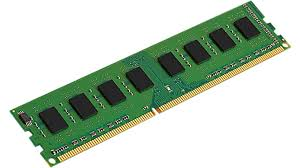
\includegraphics[width=4cm]{ram.jpg}
        \centering
        \caption{ram}
        \label{fig:Memoria RAM}
        \end{figure}    
        
        
        \subsubsection{Memoria cache}
        Una memoria mucho mas rapida que la memoria RAM, se divide en tres niveles L1, L2 y L3, y es allí donde se lleva la información mas usada en el computador. Se encuentra en nucleo del computador y su principal problema es el costo de producción, al ser tan alto es poco viable incomporarlas en grandes cantidades en los computadores hogareños.   
        
        \subsubsection{Memoria virtual}
        se trata de una porción de disco duro donde se almacena aplicaciones en ejecutación y que no ocupan tanto espacio, estas aplicaciones estan listas para ser usadas en cualquier comemnto sin ocupar espacios innecesarios en la memoria RAM.  
        
        \subsubsection{memoria disco duro}
        la Memoria de Disco duro o memoria no volatil se encarga de guardar los datos que la memoria RAM elimina una vez se dejaron de usar, la capacidad de lectura  escritura es muchisima mas pequeña que la capacidad que tiene la memoria RAM
        
        (\ref{fig:discoDuro})
        \begin{figure}[h]
        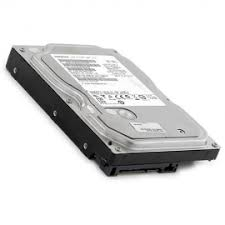
\includegraphics[width=4cm]{discoDuro.jpg}
        \centering
        \caption{Disco Duro}
        \label{fig:discoDuro}
        \end{figure}
        
        
        \subsubsection{Memorias Flash}
        Son memorias hechas a partir de del uso de semiconductores no volatiles y re-escribibles, utiles que permite la lectura y escritura de multiples posiciones de memoria en la misma operación, esto otorga una gran velocidad de funcionamiento sobre las memorias tipo ROM. Una de sus ventajas más importantes es el bajo costo y su aumento de capacidad, ademas de su bajo consumo de energia y su portabilidad 
        
        (\ref{fig:flash})
        \begin{figure}[h]
        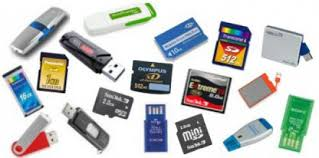
\includegraphics[width=4cm]{flash.jpg}
        \centering
        \caption{Memoria Flash}
        \label{fig:flash}
        \end{figure}
    
    
    \subsection{describa la manera como se gestiona la memoria en un computador}
    La gestión de la memoria se hace a través de microprocesadores que saca la información o los datos y los lleva del disco duro a la memoria donde se  leen y se modifica a gusto del usuario, luego de terminar el proceso con los datos estos mismos microprocesadores llevan la información modificada a el disco duro mediante el bus de datos, en el disco duro los microprocesadores sobrescriben el mismo archivo, con esto se reemplaza por el archivo viejo por el nuevo. 
    El archivo es eliminado de la memoria RAM para evitar que ocupe espacio innecesario, con esto se puede asignar espacio a la memoria a otros procesos que necesiten, que igualmente lo liberaran cuando ya no lo requieran, de esta gestión se encarga el sistema operativo, ciertamente lo hace el administrados de memoria y su labor consiste en llevar el registro de las aplicaciones que necesitan memoria, la cantidad que necesitan y cuando ya no necesitan memoria.
 
    
    
    \subsection{¿Qué hace que una memoria sea más rápida que otra? ¿Por qué esto es importante?}
    La capacidad de almacenamiento sin duda alguna es un aspecto del cual se puede partir para comparar dos memorias, por ejemplo una memoria de 4 GB será más lenta que una memoria de 8 GB, también hay que tener en cuenta los ciclos, dos memorias de 4 GB van a ser diferentes si una trabaja a 3GHz y otra a 6Ghz por lo que estos dos aspectos principalmente hacen que una memoria sea más rápida que otra. Esto es importante porque una memoria más rápida permite hacer tareas mucho más exigentes de maneras mucho más eficientes. 


\section{Conclusión} \label{conclulsion}



\bibliographystyle{IEEEtran}
\bibliography{references}
\end{document}